\documentclass{sp}

% The \pdf* commands provide metadata for the PDF output.
% Do not use LaTeX style / commands like \emph{} inside these.
\pdfauthor{Author Full Name(s)}
\pdftitle{Full title}
\pdfkeywords{adjective ordering, subjectivity, hierarchical structure, modification, reference resolution}

% Optional short title inside square brackets, for the running headers.
% If no short title is given, no title appears in the headers.
%\title[Adjective ordering preferences]{On the grammatical source of adjective ordering preferences%
\title[On the grammatical source of adjective ordering preferences]{On the grammatical source of adjective ordering preferences%
	\thanks{We gratefully acknowledge the feedback we received on earlier drafts from Kjell Johan S\ae b\o\  and two anonymous reviewers. Special thanks go to Michael Franke for very helpful discussions.}}

% Optional short author inside square brackets, for the running headers.
% If no short author is given, no authors print in the headers.
\author[Scontras, Degen, Goodman]{% As many authors as you like, each separated by \AND.
	\spauthor{Gregory Scontras \\ \institute{University of California, Irvine}} \AND
	\spauthor{Judith Degen \\ \institute{Stanford University}} \AND
	\spauthor{Noah D. Goodman \\ \institute{Stanford University}}}

	

\usepackage{linguex}
\usepackage{qtree}
\qtreecenterfalse
\usepackage{tree-dvips}
\usepackage{phonetic}
\usepackage{xcolor}
\usepackage{pifont}
\usepackage{lineno}
\usepackage{graphicx}
%\usepackage{qdotbranch}
\usepackage{booktabs}
\usepackage{multirow}
\usepackage{CJK}
\usepackage{tikz}
\usepackage{amsfonts} 
\usepackage{amsmath}
\usepackage{hyperref}

\def\url#1{\expandafter\string\csname #1\endcsname}

\definecolor{Blue}{RGB}{0,0,255}
\newcommand{\jd}[1]{\textcolor{Blue}{[jd: #1]}}  
\newcommand{\gcs}[1]{\textcolor{blue}{[gcs: #1]}}  


\newcommand{\type}[1]{\ensuremath{\left \langle #1 \right \rangle }}
\newcommand{\lam}{\ensuremath{\lambda}}

\renewcommand{\firstrefdash}{}

\begin{document}

\maketitle

\begin{abstract}
	\cite{scontrasetal2017adjectives} present experimental evidence demonstrating that the best predictor of adjective ordering preferences in the English noun phrase is the subjectivity of the property named by any given adjective: less subjective adjectives are preferred linearly closer to the nouns they modify. The current work builds on this empirical finding by proposing that the reason subjectivity predicts adjective ordering preferences has to do with the hierarchical structure of nominal modification. Adjectives that are linearly closer to the modified noun are often structurally closer, composing with the noun before adjectives that are farther away. Pressures from successful reference resolution dictate that less subjective, more useful adjectives contribute their meaning to the resulting nominal earlier, in an attempt to more effectively limit the reference search space.
\end{abstract}

\begin{keywords}
	adjective ordering, subjectivity, hierarchical structure, modification, reference resolution
\end{keywords}

\section{Introduction}

Adjective ordering preferences determine the relative order of adjectives in multi-adjective strings. Such preferences dictate that \emph{small brown cardboard box} sounds much more natural than \emph{brown cardboard small box}, or any other ordering of the adjectives. 
These preferences are robustly attested, not only in English, but in a host of unrelated languages \citep[see, among others,][]{dixon1982}. Remarkably, the \emph{same} preferences surface in each case. Even more remarkably, in post-nominal languages where adjectives follow modified nouns, the preferences are the mirror image of what are found in pre-nominal languages like English; %\citep{dixon1982,hetzron1978,sproatshih1991}; 
at issue is the relative distance of an adjective from the noun it modifies.

Given their stability within and across languages, a glaring question presents itself: what factors determine these robust preferences? Answers to this question stand to inform not only the preferences, but also the psychological and grammatical systems from which these preferences emerge. For this reason, adjective ordering preferences have been the subject of targeted inquiry since \cite{sweet1898} wrote about them over a century ago. Hypotheses abound, ranging from the psychological \citep[e.g.,][]{whorf1945,martin1969} to the grammatical \citep[e.g.,][]{cinque1994,mcnallyboleda2004,truswell2009}. Still, significant progress has proven elusive, owing to the complex empirical work required to test these hypotheses.

Recently, \cite{scontrasetal2017adjectives} brought behavioral and corpus data to bear on the question of adjective ordering. Distilling the proposals that preceded them, \citeauthor{scontrasetal2017adjectives} advanced the hypothesis that property subjectivity determines the relative order of adjectives in multi-adjective strings, such that less subjective adjectives occur linearly closer to the nouns they modify (see also \citealp{hetzron1978,tucker1998,hill2012}). In \emph{the small brown cardboard box}, \emph{cardboard} is less subjective than \emph{brown} or \emph{small}, so \emph{cardboard} is preferred closer to the modified noun.

%With strong empirical footing for the factor determining ordering preferences, the current paper addresses the question of precisely \emph{why} subjectivity should play such a central role in adjectival modification. The proposal offered ties subjectivity to reference resolution and the hierarchical structure of adjectival modification.


With strong empirical footing for the factor determining ordering preferences, the current paper addresses the question of precisely \emph{why} subjectivity should play such a central role in adjectival modification. Section \ref{review} reviews the empirical methodology and findings from \cite{scontrasetal2017adjectives}. Section \ref{why} explores potential explanations of the empirical findings. Section \ref{proposal} offers a proposal tying subjectivity to reference resolution and the hierarchical structure of adjectival modification. Section \ref{conclusion} concludes.


\section{Subjectivity predicts adjective ordering preferences} \label{review}

To identify the factors at play in adjective ordering preferences, we must first determine what the preferences are that need explaining. To that end, \cite{scontrasetal2017adjectives} established a behavioral measure of ordering preferences. Experimental participants indicated the preferred ordering of adjectives in adjective-adjective-noun strings (e.g., \emph{the small brown chair} vs. \emph{the brown small chair}), which yielded a single preferred-distance measure for each adjective tested.
% From these relative preferences the authors then calculated a single preferred-distance measure for each adjective tested, corresponding to that adjective's overall proximity to modified nouns. 
The authors evaluated their behavioral proximity measure against naturalistic productions from English corpora. Finding an extremely strong correlation between the behavioral measure and the corpus counts ($r^2 = .83$), the authors concluded that na\"ive speakers have reliable and robust adjective ordering preferences, and that the behavioral measure faithfully captured these preferences. The authors then shifted their focus to the aspect of adjective meaning that they hypothesized best predicted ordering preferences: subjectivity. 

Inspired by various proposals about aspects of adjective meaning explaining their relative order in multi-adjective strings, \citeauthor{scontrasetal2017adjectives} distilled past proposals into the intuitive psychological construct of subjectivity. Crucially, the authors \emph{operationalized} their subjectivity hypothesis as a behavioral measure for the purpose of empirical testing. Adjective subjectivity was measured by asking participants how ``subjective'' a given adjective was. These raw ``subjectivity'' scores were evaluated against a potentially more ecologically valid method: faultless disagreement \citep[e.g.,][]{kolbel2004,macfarlane2014}. To the extent that two speakers can disagree about a given property for an object without one speaker necessarily being wrong (e.g., disagreeing about whether or not a box counts as small), the property admits that degree of faultless disagreement, which stands proxy for the adjective's subjectivity. Finding extremely high correlations between the ``subjectivity'' scores and the faultless disagreement measure ($r^2 = .91$), \citeauthor{scontrasetal2017adjectives} concluded that both measures successfully capture adjective subjectivity.

%\gcs{note on our operationalization of subjectivity and the various semantic factors that contribute to it} 
It bears noting that many factors can contribute to the perceived subjectivity of an adjective, including semantic notions typically thought of as vagueness (e.g., red by which standard?), evaluativity (e.g., beautiful according to whom?), or relativeness/context dependence (e.g., large compared to what?). Moreover, there exist a variety of semantic theories designed to account for these specific notions (e.g., the supervaluations of \citealt{kamppartee1995}, the perspectives of \citealt{kolbel2002}, or the judges of \citealt{lasersohn2005}). There are also various formal notions of the subjective vs. objective distinction defined in terms of judges \citep{saebo2009}, counterstances \citep{kennedywiller2016}, outlooks \citep{coppock2018}, etc. For our purposes and the purposes of \citeauthor{scontrasetal2017adjectives}'s study, the semantic source of subjectivity runs orthogonal to the simple fact that speakers have stable estimates of subjectivity operationalized via faultless disagreement. In other words, whatever its source, language users recognize that certain adjectives can lead more frequently to cases of misalignment where people might (faultlessly) disagree about the set of things picked out by a given adjective. It is this notion that we refer to with the label ``subjectivity''.

With clear estimates of adjective subjectivity and of the preferences themselves, the authors then tested the predictive power of subjectivity in explaining ordering preferences. %Recall the hypothesis: adjectives with lower subjectivity scores are preferred linearly closer to the nouns they modify. Indeed, this is precisely what 
\citeauthor{scontrasetal2017adjectives} found that an adjective's semantics does predict its distance from the nouns it modifies, with subjectivity scores accounting for nearly all of the variance in the ordering preference data. Moreover, preference strength increased with the subjectivity differential. To get a clearer picture of the \emph{relative} success of their subjectivity hypothesis, the authors then compared the predictions of subjectivity against operationalizations of competing proposals: adjective inherentness (whereby adjectives with more ``essential'' meanings occur closer to modified nouns; \citealp[e.g.,][]{whorf1945}), intersective vs. subsective modification (whereby intersective modifiers compose first in the hierarchical structure of nominals; \citealp{truswell2009}), and concept formability (whereby adjectives that form complex, idiomatic concepts compose early; \citealp[e.g.][]{mcnallyboleda2004}). In each case, subjectivity continued to be a better predictor of ordering preferences.


\section{Why subjectivity?} \label{why}

Finding subjectivity to be a reliable and robust predictor, our task now is to explain why subjectivity should determine adjective ordering preferences: why should less subjective adjectives be preferred linearly closer to the nouns they modify? \citeauthor{scontrasetal2017adjectives} hint at an answer in the discussion of their results, namely pressure from successful reference resolution. Before reviewing their discussion, it will be useful to first consider the range of possible answers to this \emph{why} question. In the process, we also establish desiderata for successful answers.

To begin, we might propose that the observed subjectivity gradient emerges from a rigid syntax of adjectival modification: adjectives inhabit specialized syntactic projections depending on their semantic class (e.g., Color Phrase for color adjectives, Shape Phrase for shape adjectives, etc.; \citealp{cinque1994,scott2002}), and these projections happen to order in a way that tracks subjectivity. While a cartographic approach along these lines might help to explain the observed behavior, it leaves unanswered the question of \emph{why} subjectivity should matter in the ordering of adjectival projections. Also problematic is the rigidity introduced by a syntax that allows only one ordering for any string of adjectives. This rigidity predicts categorical ordering preferences, yet \citeauthor{scontrasetal2017adjectives} observed graded judgments that track differential subjectivity. Thus, a cartographic syntax appears to be a nonstarter for explaining why subjectivity should predict ordering preferences.

Shifting our sights to psychological explanations, we might try to account for subjectivity by appealing to the relative salience of properties for the nouns they modify. Properties that are more salient\dash more \emph{inherent} to the objects described by the noun \citep[e.g.,][]{whorf1945}\dash ought to be more accessible in the construction of nominals. An account based on the accessibility of adjectives during the on-line construction of nominal phrases stands to extend straightforwardly to languages with post-nominal adjectives where the preferences are preserved in the reverse: phrases are built outward from their heads, so more accessible adjectives occur linearly closer to the head of the nominal construction (i.e., the noun). The leap that must be made links subjectivity to inherentness and thereby to accessibility. Unfortunately, this leap appears untenable. \citeauthor{scontrasetal2017adjectives} measured adjective inherentness and compared its predictions with those of subjectivity. Whereas subjectivity accounted for at least 75\% of the variance in the ordering preferences, inherentness accounted for 0\%. While an explanation in terms of adjective accessibility might still prove promising, the implementation via inherentness lacks empirical support.

Rather than inherentness, we might try tying adjective accessibility to adjective frequency, such that more frequent adjectives are more accessible during the hierarchical construction of nominal phrases. To account for the role of subjectivity, we would expect more frequent\dash and thus more accessible\dash adjectives to have lower subjectivity scores. \citeauthor{scontrasetal2017adjectives} investigated the role of adjective frequency in ordering preferences, finding it to be a significant predictor. However, frequency applies pressure in the direction opposite to what we have been considering: in English, more frequent adjectives occur \emph{farther} from the noun because they occur \emph{linearly} early in multi-adjective strings \citep[cf.][]{wulff2003}. 
Moreover, the authors found that subjectivity continued to explain significant variance in the preferences over and above adjective frequency. While frequency likely contributes to the relative accessibility of adjectives, its contribution is separate from that of subjectivity; the two forces work in tandem and in orthogonal directions. %\jd{\emph{I find it a little odd to say that they work in opposite directions -- that would only be true if in general more subjective adjectives were generally low-frequency. It's more that these are two orthogonal forces, no?}} %We can see the two pressures pull apart once we consider specific examples. Material adjectives like \emph{wooden} or \emph{metal} were found to be the least subjective in \citeauthor{scontrasetal2017adjectives}'s study; value adjectives like \emph{good} and \emph{bad} were the most subjective.   Thus, accessibility by frequency does little to explain why subjectivity should play such a central role.

We find perhaps the most thought-through version of the psychological accessibility hypothesis in \citeauthor{martin1969competence}'s (\citeyear{martin1969competence}) experimental investigations. Inspired by prior results demonstrating the predictive power of ``definiteness of denotation'' in adjective ordering preferences \citep{martin1969}, \citeauthor{martin1969competence} set out to test the hypothesis that adjectives occurring linearly closer to nouns indeed are more accessible. Participants completed a series of elicited production tasks in which they observed visual arrays of objects and named specific properties of the objects they saw (e.g., size vs. color). There were two versions of the experiments: one for English speakers, and another for speakers of Indonesian, a post-nominal language with the mirror image of the English preferences. By measuring production latencies, \citeauthor{martin1969competence} discovered that adjectives preferred linearly closer to nouns are produced more quickly. From this he concluded that adjectives closer to the noun are more accessible than adjectives farther away. 

Before accepting \citeauthor{martin1969competence}'s results as unambiguous support for an adjective accessibility hypothesis, we must confront two issues. First, production latencies in context likely depend on more than the relative accessibility of words from memory; how can we be sure that the observed differences in latencies did not derive from low-level properties of the visual displays? If the issue at play is truly the \emph{lexical} accessibility of adjectives, then the displays should have controlled for the relative perceptual salience of the properties being named. As things stand, we have no way of teasing apart lexical accessibility from visual salience in \citeauthor{martin1969competence}'s results.
%If ordering preferences depend on the relative salience of various adjectives during the on-line construction of a nominal phrase, then there should be contexts in which canonical orderings are reversed. 
Second, if accessibility truly determines adjective ordering preferences, why should adjective frequency apply pressure in the opposite direction? Relative frequency surely determines adjective accessibility, and we saw that adjective frequency is a significant predictor of ordering preferences. However, more frequent adjectives are preferred early in the linear structure of nominal phrases, not closer to the nominal head (at least not in pre-nominal languages like English). Accessibility as measured by adjective frequency seems to be delivering the wrong predictions.


%% MARTIN 1969 COMPETENCE
%"it is hypothesized that the left-to-right order of morphemes in the bases corresponds to the habitual real time order of choice of these morphemes."
%"it is hypothesized that the left-to- ight reordering of morphemes by transform- ations corresponds to the habitual reordering of those morphemes in real time for pro- duction"
%"It is therefore proposed that speakers of English and Indonesian habitually choose adjectives after choosing the modified nouns"
%"in English, preferred adjective order should correlate negatively with the order of adjective choice and, in Indonesian, the correlation should be positive."
%"adjectives preferred close to the noun are generally
%capable of stronger associations with the noun"
%"produce the appropriate value for the dimension presented to them as quickly as possible. Thus, if they had been instructed to attend to LARGE RED CIRCLE and had been given the word size, it was their task to respond with the word large as quickly as possible. By recording the latencies of these encoding responses, it was possible to determine the relative accessibilities of the adjectives involved."
%"Lockhart and Martin have shown that the adjectives which are expressed first in English are less available for recall than those which are expressed later."
%Adjectives closer to the noun are more "Accessible"

%% MARTIN 1969 DETERMINANTS
%"the proper choice of an adjective often depends on a relation- ship between the meaning of the modified noun and the property to be denoted by the adjective"
%"adjectives differ in the degree to which the noun context must be considered in the choice of adjectives"
%"The accessibility of adjectives is hypothesized to depend, in part, on the degree to which their choice is constrained by the meaning of the modified noun. In the choice of those adjectives which are context inde- pendent in denotations, less time is thought to be required for scanning the meaning of the modified noun than in the choice of adjectives which are context-sensitive in denotation."
% This is really just codifying the intersective vs. subsective distinction
%"If an adjective is frequently used in many different contexts, its user will be more sensi- tive to the ways in which its meaning is affected by noun context than if the adjective is infrequently used."
%"when Ss were given ample time to judge the definite- ness or absoluteness of adjectives, frequency did not significantly correlate with those judgments"


There of course remains the possibility that accessibility is not the primary link between subjectivity and ordering preferences. In an attempt to tie properties of language structure to general principles of cognition, \cite{bever1970} advanced the hypothesis that structural norms\dash among them, adjective ordering preferences\dash emerge from the human perceptual system. To see how perception could determine the preferred ordering of adjectives, one must appreciate the task of the parser, at least as envisaged by \citeauthor{bever1970}. Upon encountering the speech stream, the parser relies on heuristics to efficiently identify constituents and associate them with an appropriate argument structure. In service of this task, the parser needs an identification mechanism for noun phrases: where do they begin, and where do they end? 

According to \citeauthor{bever1970}, the more ``nounlike'' the adjective, the closer it appears to the modified noun. %\citep[see also][]{biberetal1999,posner1986}. 
Returning to the small brown cardboard box, \emph{cardboard} is the most felicitous when used as a noun, \emph{brown} slightly less so, and \emph{small} the least of all (cf. \citeauthor{bever1970}'s examples (68) and (69)). 
%(modified from \citeauthor{bever1970}'s examples (68) and (69)):
%
%\ex. \a. Brown is a color.
%\b. Cardboard is a material.
%\b. *That box is made out of brown.
%\b. That box is made out of cardboard.
%\b. *The brown broke.
%\b. The cardboard broke.
%
%\ex. \a. Brown is my favorite color.
%\b. *Small is my favorite size.
%\b. He splattered some brown on me.
%\b. *He splattered some small on me.
%\b. Brown and blue and green are colors.
%\b. ?Small and large and enormous are sizes.
%
Now, why should ordering adjectives according to their nounlike character ease the burden of the parser in its search for noun phrase boundaries? \citeauthor{bever1970} proposes that a linear parser identifies the beginning of a noun phrase with the presence of a determiner. That same parser identifies the right edge of the noun phrase with the transition from a clearly nounlike element to an item that is ``less uniquely a noun'' \pgcitep{bever1970}{323}. In other words, the primary cue to the right edge of a noun phrase is a salient decrease in nounlike character. If adjectives were randomly ordered with respect to their nounlike character, the parser might mistakenly identify noun phrase boundaries, as in [\emph{the cardboard}] [\emph{brown box}]. These early errors identifying phrase boundaries would cascade into a total failure for the sentence parse.

\citeauthor{bever1970}'s proposal offers an intuitive explanation of the pressures that determine pre-nominal adjective ordering, and it might extend to handle the mirror-image preferences in post-nominal languages. The proposal even offers a promising connection to subjectivity: perhaps less subjective adjectives yield more-well-defined categories, which are more amenable to naming with nouns. Thus, subjectivity determines nounlike character, and nounlike character determines ordering preferences. Unfortunately, \citeauthor{bever1970}'s proposal suffers a serious flaw: it lacks empirical support. In her corpus analysis of English ordering preferences, \cite{wulff2003} %p.255
calculated nounlike character and demonstrated that it does little by way of predicting adjective order. What effect nounlike character does have on the linear order of adjectives applies pressure in the direction opposite of \citeauthor{bever1970}'s hypothesis: more nounlike adjectives are marginally more likely to occur \emph{farther} from the modified noun \pgcitep{wulff2003}{255}.

It would appear that we have arrived at an impasse: accessibility-based accounts struggle to explain the full range of data from both pre- and post-nominal languages; they also face a serious obstacle in the form of lexical frequencies. \citeauthor{bever1970}'s perception-based account seems well-suited for pre- and post-nominal languages, but \citeauthor{wulff2003}'s facts suggest the proposal is misguided. And all of these proposals lack a clear connection to adjective subjectivity. There remains another strategy, however, which shifts the explanation from how language users use adjectives to what adjectives do for language users. As we shall see, a functional account along these lines stands the best chance of explaining the role of subjectivity in determining ordering preferences.

For \cite{seiler1978}, the clue to understanding ordering preferences lies in the task that adjectives perform: determination. Noun phrases are inherently referential, whether to real-world objects or to well-defined concepts. In either case, determiners in the broad sense\dash demonstratives, articles, numerals, quantifiers, adjectives, prepositional attributes, relative clauses\dash contribute to nominal meaning in service of pinning down a referent. With this function in mind, \citeauthor{seiler1978} identifies regularities in the linear order of determiners. First, ``the range of head nouns for which a determiner D is potentially applicable increases with the positional distance of that determiner from the head noun N'' \pgcitep{seiler1978}{308}. For the purposes of adjective ordering, the more nouns an adjective can felicitously describe, the farther that adjective will appear from the noun. \citeauthor{seiler1978} explicitly links determiner applicability with property inherentness: less broadly-applicable, more special-purpose adjectives name properties that are more inherent to the modified noun. He gives the example of \emph{rote h\"{o}lzerne Kugeln} `red wooden balls':

\begin{quotation}The semantic structure of \emph{Kugeln} qua solid objects naturally implies material constitution of some sort; it implies\dash with a lesser degree of naturalness\dash some property in the color spectrum. To this gradient decrease in natural semantic implication corresponds the normal word order in which the `determiner' with the strongly implied property is closer to the head noun than the `determiner' with the less strongly implied property. \pgcitep{seiler1978}{309}\end{quotation}

Properties implied by the nominal have meanings that are at least partially contained already within the nominal meaning, hence the implication (cf. the notion of mutual informativity; \citealp{futrell2017}). Determiners that are less implied by the nominal will be more informative (i.e., unexpected) when encountered, with greater informativity leading to a greater potential of pinning down the intended referent.  Thus, according to \citeauthor{seiler1978}, ``the potential of a determiner D for singling out the object referred to by the head noun N increases proportionally with the positional distance of D from N'' \pgcitep{seiler1978}{309}. The ordering that results presumably follows from the desire to introduce the more informative, more useful elements early in the construction of a nominal.

\citeauthor{seiler1978}'s first claim\dash that adjectives describing a broader set of nouns appear farther from the modified noun\dash finds empirical support in \citeauthor{wulff2003}'s corpus analysis \pgcitep{wulff2003}{266--267}. However, the implication of \citeauthor{seiler1978}'s second claim\dash that speakers introduce more useful elements (for the purpose of determination) earlier\dash fails in the case of post-nominal languages with mirror-image preferences. This reasoning would hold that speakers in post-nominal languages save the most useful adjectives for last, which stands in direct conflict with the explanation for pre-nominal languages. Still, we should not abandon the functional account of adjective ordering altogether. In the following section, we consider a different proposal that preserves \citeauthor{seiler1978}'s intuition that ``in order to fully understand the regularities we must look behind the mere facts and try to see the program and ultimately the purposive functions of which they are manifestations'' \pgcitep{seiler1978}{325}.

%% Seiler 1978 on ``determination''
%
%problem: mirror image preferences
%

%
%"The more widely a 'determiner' is applicable to a head noun (AI), the more it contributes to determining the reference and the less it contributes to determining the concept of the head noun (A2). The less widely applicable a 'determiner', the less it contributes to reference (AI), and the more it contributes to identifying the
%concept (A2). explicating, as it were, its inherent properties." p. 310
%
%Behagel's first law
%
%"evaluating adjectives surpass color and material adjec- tives in distance with respect to N because their specificatory function (i.e, the function which determines reference or extension) outweighs their char- acterizing function (l.e. the function which determines properties of the concept or intension)" p. 311
%
%"potential for "pinning down" a referent" p. 313
%
%"local squishiness" p.314
%
%"In order to fully understand the regularities we must look behind the mere facts and try to see the program and ultimately the purposive functions of which they are manifestations" p.325

\section{Linking subjectivity to the hierarchical structure of modification} \label{proposal}

Let us begin as \citeauthor{seiler1978} did, with the observation that adjectives aid in establishing reference. Starting with a noun like \emph{box}, potential referents include every box in the discourse context. Where there are multiple boxes, the listener's task of establishing reference amounts to a game of chance. We increase our odds of winning this game as we narrow down, or \emph{determine} the set of potential referents. Encountering an adjective like \emph{cardboard}, we now only consider the subset of boxes that are cardboard. Encountering \emph{brown}, we limit ourselves to the cardboard boxes that are brown. Encountering \emph{small}, we further limit ourselves to just those brown cardboard boxes that are small. From the set of all boxes we home in on the small brown cardboard boxes, a much smaller set indeed.

When it comes to the structure of these multi-adjective strings, we treat adjectival modification as syntactic adjunction, as in \ref{modification}. Semantically, we treat modification as set intersection, where the adjective restricts the set characterized by the nominal denotation to just those elements that hold the specified property. For our purposes, it does not matter whether this intersection proceeds via a special mode of semantic composition (e.g., Predicate Modification; \citealp{heimkratzer1998}), via functional application with adjectives of a higher type \citep[e.g.,][]{parsons1970modifiers},
%{parsons1970modifiers,montague1970,kamp1975,siegel1976}, 
or via functional structure \citep[e.g.,][]{scontrasnicolae2014}. In each case, semantic composition proceeds outward from the noun; adjectives closer to the noun make their semantic contribution earlier than adjectives farther away. The resulting nominal denotation appears in \ref{denotation}, where the full NP characterizes the set of small brown cardboard boxes.

\ex. \label{modification}
\Tree [.NP [.AP \emph{small} ] [.NP$_3$ [.AP \emph{brown} ] [.NP$_2$ [.AP \emph{cardboard} ] [.NP$_1$ \emph{box} ] ] ] ] 

\ex. \label{denotation}
\sv{\text{small brown cardboard box}} = \flushright \mbox{\lam x. box(x) = cardboard(x) = brown(x) = small(x) = 1}

\begin{figure}[t]
	\centering
	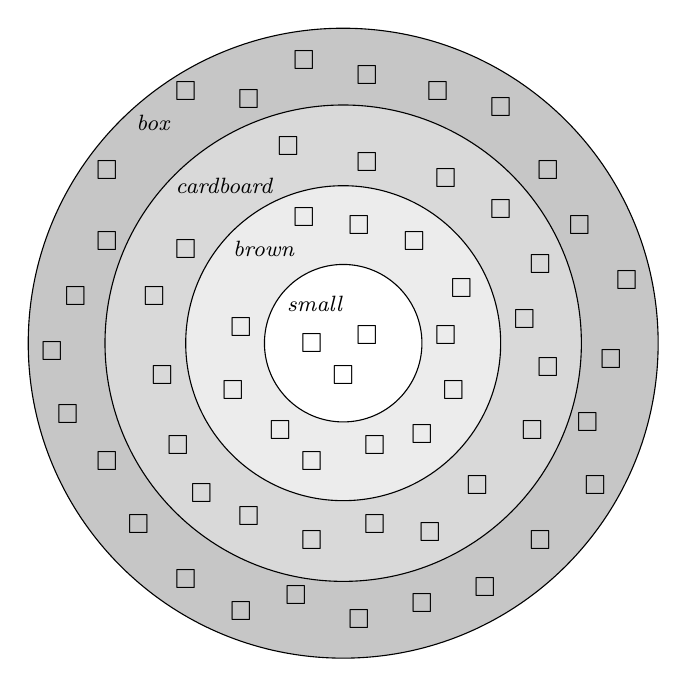
\begin{tikzpicture}
	%                              \draw (-2, 1.2) rectangle (2, -2.2);
	\begin{scope}
	\clip (0, 0) circle (4);
	\fill[color=gray!45] (-5,5)
	rectangle (5,-5);    
	\end{scope}
	\begin{scope}
	\clip (0, 0) circle (3.025);
	\fill[color=gray!30] (-5,5)
	rectangle (5,-5);    
	\end{scope}
	\begin{scope}
	\clip (0, 0) circle (2);
	\fill[color=gray!15] (-5,5)
	rectangle (5,-5);    
	\end{scope}
	\begin{scope}
	\clip (0, 0) circle (1);
	\fill[color=gray!0] (-2,1.5)
	rectangle (2,-1.5);    
	\end{scope}
	\node(a) at (-0.35,.5) {\footnotesize\emph{small}}; %%% 3 boxes
	\node(a) at (0,-.4) {$\Box$};
	\node(a) at (0.3,.1) {$\Box$};
	\node(a) at (-0.4,0) {$\Box$};
	\node(a) at (-1,1.2) {\footnotesize\emph{brown}}; %%% 12 boxes
	\node(a) at (-.5,1.6) {$\Box$};
	\node(a) at (.2,1.5) {$\Box$};
	\node(a) at (.9,1.3) {$\Box$};
	\node(a) at (1.5,.7) {$\Box$};
	\node(a) at (1.3,.1) {$\Box$};
	\node(a) at (1.4,-.6) {$\Box$};
	\node(a) at (1,-1.15) {$\Box$};
	\node(a) at (0.4,-1.3) {$\Box$};
	\node(a) at (-0.4,-1.5) {$\Box$};
	\node(a) at (-0.8,-1.1) {$\Box$};
	\node(a) at (-1.4,-.6) {$\Box$};
	\node(a) at (-1.3,.2) {$\Box$};
	\node(a) at (-1.5,2) {\footnotesize\emph{cardboard}}; %%% 18 boxes
	\node(a) at (-2,1.2) {$\Box$};
	\node(a) at (-2.4,.6) {$\Box$};
	\node(a) at (-2.3,-.4) {$\Box$};
	\node(a) at (-2.1,-1.3) {$\Box$};
	\node(a) at (-1.8,-1.9) {$\Box$};
	\node(a) at (-1.2,-2.2) {$\Box$};
	\node(a) at (-.4,-2.5) {$\Box$};
	\node(a) at (0.4,-2.3) {$\Box$};
	\node(a) at (1.1,-2.4) {$\Box$};
	\node(a) at (1.7,-1.8) {$\Box$};
	\node(a) at (2.4,-1.1) {$\Box$};
	\node(a) at (2.6,-.3) {$\Box$};
	\node(a) at (2.3,.3) {$\Box$};
	\node(a) at (2.5,1) {$\Box$};
	\node(a) at (2,1.7) {$\Box$};
	\node(a) at (1.3,2.1) {$\Box$};
	\node(a) at (.3,2.3) {$\Box$};
	\node(a) at (-.7,2.5) {$\Box$};
	\node(a) at (-2.4,2.8) {\footnotesize\emph{box}}; %%% 26 boxes
	\node(a) at (-3,2.2) {$\Box$};
	\node(a) at (-3,1.3) {$\Box$};
	\node(a) at (-3.4,.6) {$\Box$};
	\node(a) at (-3.7,-.1) {$\Box$};
	\node(a) at (-3.5,-.9) {$\Box$};
	\node(a) at (-3,-1.5) {$\Box$};
	\node(a) at (-2.6,-2.3) {$\Box$};
	\node(a) at (-2,-3) {$\Box$};
	\node(a) at (-1.3,-3.4) {$\Box$};
	\node(a) at (-.6,-3.2) {$\Box$};
	\node(a) at (0.2,-3.5) {$\Box$};
	\node(a) at (1,-3.3) {$\Box$};
	\node(a) at (1.8,-3.1) {$\Box$};
	\node(a) at (2.5,-2.5) {$\Box$};
	\node(a) at (3.2,-1.8) {$\Box$};
	\node(a) at (3.1,-1) {$\Box$};
	\node(a) at (3.4,-.2) {$\Box$};
	\node(a) at (3.6,.8) {$\Box$};
	\node(a) at (3,1.5) {$\Box$};
	\node(a) at (2.6,2.2) {$\Box$};
	\node(a) at (2,3) {$\Box$};
	\node(a) at (1.2,3.2) {$\Box$};
	\node(a) at (.3,3.4) {$\Box$};
	\node(a) at (-.5,3.6) {$\Box$};
	\node(a) at (-1.2,3.1) {$\Box$};
	\node(a) at (-2,3.2) {$\Box$};
	
	\draw (0, 0) circle (1);
	\draw (0, 0) circle (2);
	\draw (0, 0) circle (3.025);
	\draw (0, 0) circle (4);
	\end{tikzpicture}
%	\includegraphics[width=3.5in]{bullseye.eps}
	\caption{An illustration of restrictive modification in \emph{small brown cardboard box}.}\label{mod-fig}
\end{figure}


To see how we arrive at the denotation in \ref{denotation}, consider the illustration of this process in Figure \ref{mod-fig}. Each circle corresponds to the denotation of an NP node in \ref{modification}, with the elements ($\Box$) contained within that circle representing elements of the nominal denotation. The outermost circle represents the denotation of the smallest NP, \emph{box}. In this toy example, there are 59 boxes. Moving inward, we arrive at the next-highest NP denotation, \emph{cardboard box}; there are only 33 such boxes, so the 26 boxes that are not cardboard are pruned from the denotation. Moving inward still, we get the 15 boxes that are both brown and cardboard; the 18 non-brown cardboard boxes have been discarded. Finally, at the innermost circle, we have just those three boxes that are at once cardboard, brown, and small; the 12 brown cardboard boxes that are not small get ignored.

Thinking about the contributions of the adjectives in the example above, we notice that, for the purpose of establishing reference, different adjectives do different amounts of work. Here, ``work'' gets equated with reference-establishing potential, or potential for information gain. Measured in terms of the number of possible referents considered, more work is done by the adjectives closer to the noun. In Figure \ref{mod-fig}, %\emph{cardboard} makes the largest cut in the noun's denotation, pruning 26 adjectives. Put differently, 
\emph{cardboard} operates over the largest set: for each of the 59 boxes, one must decide whether or not it is cardboard. Thus, there are 59 opportunities to make a mistake in this decision process, wherein a listener might misjudge a box as cardboard or not. The next adjective, \emph{brown}, operates only over the 33 cardboard boxes; thus, there are fewer possibilities for error. The last adjective, \emph{small}, operates over the smallest set, with the smallest chance of error.

Here is the crux of the account, and finally a return to the issue of subjectivity: less subjective content is more useful for effectively communicating about the world (i.e., establishing reference). %\jd{\emph{Instead of "communicating about the world" can we say "establishing reference"? Because it's not clear that it's true otherwise -- in particular, I learn a lot more about a speaker from their use of subjective adjectives than from their use of objective adjectives.}} 
Encountering a relatively objective adjective like \emph{cardboard}, a listener arrives at a precise concept\dash one that closely aligns with that of the speaker who uttered the adjective. More subjective adjectives introduce the potential for errors in alignment, as speakers and listeners might (faultlessly) disagree about category boundaries. When it comes to ordering preferences, speakers consolidate the less subjective, more useful content around the modified noun. The claim is that they do so in an attempt to aid the listener in establishing reference by minimizing errors in alignment. 

The following subsection walks through concrete examples of how ordering with respect to decreasing subjectivity minimizes alignment errors and maximizes the probability of successful referent classification. Having demonstrated the utility of subjectivity-based ordering, we then discuss potential worries and further avenues to explore.

\subsection{A mathematical demonstration}

To get our story off the ground, we must consider the semantics of modification in more detail. To model the potential for faultless disagreement in subjective properties, we introduce noise into the semantics of our adjectives. 
%, as in \ref{noisy-sem}. The function \texttt{flip(x)} returns a sample from a Bernoulli distribution, where a random variable takes the value 1 with probability \texttt{x}; one can think of this function as simulating the outcome of a weighted coin flip, where heads corresponds to 1 (i.e., true) and tails corresponds to 0 (i.e., false). For our purposes, the addition of \texttt{flip()} to an adjective's semantics introduces noise at the rate $\epsilon$, where $\epsilon$ increases with subjectivity. Thus, $\epsilon_{\footnotesize\textrm{cardboard}} < \epsilon_{\footnotesize\textrm{brown}} < \epsilon_{\footnotesize\textrm{small}}$.
%
%\ex. \label{noisy-sem}
%\sem{ADJ} = \lam x. if \texttt{ADJ}(x) then \texttt{flip}($1-\epsilon$), else \texttt{flip}($\epsilon$)
%
%Stacking a series of noisy adjectives together in a modification structure, there will indeed be a greater chance of incorrect classifications (i.e., misalignments) if the adjectives are not ordered according to subjectivity. %The larger the denotation with which a noisy adjective composes, the greater the opportunity for misclassifications: 
%\gcs{fuller discussion of the math}
For each potential referent an adjective classifies, we introduce the potential for misclassification $\epsilon_{adj}$, which stands proxy for the adjective's subjectivity.\footnote{A general schema for formalizing the potential for misclassification in an adjective's semantics appears in \Next: 
	\ex. \sv{\text{ADJ}} = \lam x. if \texttt{ADJ}(x) then \texttt{flip}($1-\epsilon_{adj}$), else \texttt{flip}($\epsilon_{adj}$)
	
The function \texttt{flip(x)} returns a sample from a Bernoulli distribution, where a random variable takes the value 1 with probability \texttt{x}; one can think of this function as simulating the outcome of a weighted coin flip, where heads corresponds to 1 (true) and tails corresponds to 0 (false). The addition of \texttt{flip()} to an adjective's semantics introduces noise at the rate $\epsilon$, where $\epsilon$ increases with subjectivity.} 
%As the number $N$ of potential referents increases, so too does the probability of misclassification $p(\textrm{error})$: 
%
%\setcounter{equation}{3}
%\begin{align}
%p(\textrm{error}_{adj}) &= 1 - p(\textrm{no-error}_{adj}) \nonumber\\
%&= 1 - (1-\epsilon_{adj})^N
%\end{align}
%
%Suppose $\epsilon_{\footnotesize\textrm{cardboard}} = 0.01$, so that there is a 1\% chance of incorrectly classifying an object as cardboard. Suppose further that $\epsilon_{\footnotesize\textrm{brown}} = 0.02$ and $\epsilon_{\footnotesize\textrm{small}} = 0.03$. 
%For a multi-adjective string, we can calculate the probability of \emph{any} errors in misclassification by multiplying the individual error probabilities from each adjective as in (\ref{multi-adj-eq}); crucially, $N$ will decrease as adjectives restrict the nominal denotation. 
%
%\begin{equation} \label{multi-adj-eq}
%p(\textrm{error}_{N\!P}) = 1 - (1-\epsilon_{adj_1})^{N_1}\ \cdot\ \ldots\ \cdot\ (1-\epsilon_{adj_n})^{N_n}
%\end{equation}
%Ordering with respect to subjectivity minimizes the probability of misclassifications for a multi-adjective string by ensuring that $N$ decreases as $\epsilon$ increases. In this way, a simple policy of minimizing misclassifications could result in the observed subjectivity-based ordering. 
%
%%If there are eight boxes with all possible combinations of the properties \textsc{small}, \textsc{brown}, and \textsc{cardboard}, as in Table \ref{adj-table}, $p(\textrm{error})$ for the string \emph{small brown cardboard box}
%%
%%\begin{table}
%%	\caption{} \label{adj-table}
%%	\centering
%%\begin{tabular}{r|llll}
%%	& \textsc{small} & \textsc{brown} & \textsc{cardboard} & \textsc{box} \\ \hline
%%	1 & \texttt{true} & \texttt{true} & \texttt{true} & \texttt{true} \\ 
%%	2 & \texttt{true} & \texttt{true} & \texttt{false}  & \texttt{true} \\
%%	3 & \texttt{true} & \texttt{false}  &  \texttt{true} & \texttt{true} \\
%%	4 & \texttt{true} & \texttt{false}  & \texttt{false}  & \texttt{true} \\
%%	5 & \texttt{false}  & \texttt{true} & \texttt{true} & \texttt{true} \\
%%	6 & \texttt{false}  & \texttt{true} & \texttt{false}  & \texttt{true} \\
%%	7 & \texttt{false}  & \texttt{false} & \texttt{true} & \texttt{true} \\
%%	8 & \texttt{false}  & \texttt{false}  & \texttt{false} & \texttt{true} \\
%%	\end{tabular}
%%\end{table}
%%
%%
%%\begin{align}
%%p(\textrm{error}_{NP}) &= 1 - (1-\epsilon_{adj_1})^{N_1}\ \cdot\ \ldots\ \cdot\ (1-\epsilon_{adj_n})^{N_n}  \nonumber\\
%%&= 1 - (1-0.01)^8\ \cdot\ (1-0.02)^4\ \cdot\ (1-0.3)^2
%%\end{align}
%%
%%
%%
%%$$p(\textrm{error}_{\footnotesize\textrm{small-brown-cardboard}}) = 1-  p(\textrm{no-error}_{\footnotesize\textrm{cardboard}}) \cdot p(\textrm{no-error}_{\footnotesize\textrm{brown}}) \cdot p(\textrm{no-error}_{\footnotesize\textrm{small}})$$
%
%To see the role of subjectivity-based ordering in minimizing misclassifications, consider the choice between \emph{small brown box} vs. \emph{brown small box}. Suppose there are four boxes, two of which are small, two brown, and one small and brown. 
%%\emph{small brown cardboard box} vs. \emph{cardboard brown small box}. Suppose we are in the scenario depicted in Fig. \ref{mod-fig}: there are 59 boxes, of which 33 are cardboard, 15 are brown and cardboard, and three are small, brown, and cardboard. Suppose further that the total number of small boxes is 33, as is the total number of brown boxes; the total number of small brown boxes is 15. 
%To calculate the probability of misclassifications for the two adjective orderings, we will need each adjective's potential for misclassification; we use the subjectivity scores from \cite{scontrasetal2017adjectives}: $\epsilon_{small} = 0.64$ and $\epsilon_{brown} = 0.20$.\footnote{Subjectivity scores are likely an inflated estimate of an adjective's potential for misclassification $\epsilon$; any values for $\epsilon_{small}$ and $\epsilon_{brown}$ would do so long as $\epsilon_{small} > \epsilon_{small}$.} Adjectives closer to the noun will compose earlier, and so the number $N$ of potential referents they must classify will be larger: the first adjective to compose will operate over a set of four boxes ($N_1$); the second adjective will operate over a set of two ($N_2$). As the following calculations demonstrate, ordering with respect to decreasing subjectivity results in a lower potential for misclassifications, (\ref{small-brown-eq}), than the reverse order, (\ref{brown-small-eq}).
%
%\begin{align} \label{small-brown-eq}
%p(\textrm{error}_{small\ brown\ box}) &= 1 - (1-\epsilon_{brown})^{N_1}\ \cdot\  (1-\epsilon_{small})^{N_2} \nonumber\\
%&= 1 - (1-0.20)^{4}\ \cdot\  (1-\textbf{0.64})^{\textbf{2}} \nonumber\\
%&= \textbf{0.95}
%\end{align}
%
%\begin{align} \label{brown-small-eq}
%p(\textrm{error}_{brown\ small\ box}) &= 1 - (1-\epsilon_{small})^{N_1}\ \cdot\  (1-\epsilon_{brown})^{N_2} \nonumber\\
%&= 1 - (1-\textbf{0.64})^{\textbf{4}}\ \cdot\  (1-0.20)^{2} \nonumber\\
%&= \textbf{0.99}
%\end{align}
%
%However, minimizing misclassifications and ensuring successful reference resolution are subtly differently notions. 
%
On the basis of $\epsilon_{adj}$, each adjective has some probability $p_{adj}(\texttt{obj})$ of correctly classifying some object \texttt{obj}: 

\setcounter{equation}{2}
\begin{equation}
p_{adj}(\texttt{obj}) = 1-\epsilon_{adj}
\end{equation}

\noindent
%\gcs{adding back in misclassification potential}
Stacking a series of noisy adjectives together in a modification structure, there will be a greater chance of incorrect classifications (i.e., misalignments) if the adjectives are not ordered according to subjectivity. %The larger the denotation with which a noisy adjective composes, the greater the opportunity for misclassifications: 
	%\gcs{fuller discussion of the math}
%For each potential referent an adjective classifies, we introduce the potential for misclassification $\epsilon_{adj}$. 
As the number of objects to be classified in the nominal denotation (i.e., the cardinality of the NP denotation $|\textrm{NP}|$) increases, so too does the probability of misclassification $p(\textrm{error})$:\footnote{For convenience, we identify NP with its extension, a set of objects.} 
	
\setcounter{equation}{3}
\begin{align}
p_{adj}(\textrm{error}) &= 1 - p_{adj}(\textrm{no-error}) \nonumber\\
&= 1 - (1-\epsilon)^{|\textrm{NP}|}
\end{align}
	
	%Suppose $\epsilon_{\footnotesize\textrm{cardboard}} = 0.01$, so that there is a 1\% chance of incorrectly classifying an object as cardboard. Suppose further that $\epsilon_{\footnotesize\textrm{brown}} = 0.02$ and $\epsilon_{\footnotesize\textrm{small}} = 0.03$. 
For a multi-adjective string, we can calculate the probability of \emph{any} errors in misclassification by multiplying the individual error probabilities from each adjective, as in (\ref{multi-adj-eq}); crucially, $|\textrm{NP}|$ will decrease as adjectives restrict the nominal denotation. 
	
\begin{equation} \label{multi-adj-eq}
p_{N\!P}(\textrm{error}) = 1 - (1-\epsilon_{adj_1})^{|\textrm{NP}_1|}\ \cdot\ \ldots\ \cdot\ (1-\epsilon_{adj_n})^{|\textrm{NP}_n|}
\end{equation}
Ordering with respect to subjectivity minimizes the probability of misclassifications for a multi-adjective string by ensuring that $|\textrm{NP}|$ decreases as $\epsilon$ increases. For a concrete example, suppose there are three boxes: $box_{s}$ is small but not brown, $box_{b}$ is brown but not small, and $box_{sb}$ is both small and brown. To calculate the probability of any misclassifications for the two adjective orderings \emph{small brown} vs. \emph{brown small}, we will need each adjective's potential for misclassification $\epsilon$; we use the subjectivity scores from \cite{scontrasetal2017adjectives} to set these values: 0.20 for \emph{brown} and 0.64 for \emph{small}.\footnote{These values are adopted for illustrative purposes only. Subjectivity scores are likely an inflated estimate of an adjective's potential for misclassification $\epsilon$. Still, any values for $\epsilon_{small}$ and $\epsilon_{brown}$ would do so long as $\epsilon_{small} > \epsilon_{brown}$.} As the following calculations demonstrate, ordering with respect to decreasing subjectivity, (\ref{multi-adj-eq-smallbrown}), results in a lower probability for misclassifications than the reverse order, (\ref{multi-adj-eq-brownsmall}):

\begin{equation} \label{multi-adj-eq-smallbrown}
p_{small\ brown\ box}(\textrm{error}) = 1 - (1-0.20)^{3} \cdot (1-0.64)^{2} = \textbf{0.93}
\end{equation}
\begin{equation} \label{multi-adj-eq-brownsmall}
p_{brown\ small\ box}(\textrm{error}) = 1 - (1-0.64)^{3} \cdot (1-0.20)^{2} = \textbf{0.97}
\end{equation}
%\gcs{end of misclassification potential}

However, minimizing misclassifications and correctly classifying the intended referent, thereby allowing for successful reference resolution, are subtly differently notions. If we assume a fixed misclassification potential $\epsilon$ for each adjective and a truly intersective semantics for modification, the probability of correctly classifying the intended referent once a noun has been modified by multiple adjectives does not depend on the order of the adjectives (i.e., the order of semantic composition). %To see why, consider the process of reference resolution from the perspective of the intended referent. 
Given the commutativity of noise in intersective modification, a nominal with two adjectives will correctly classify the intended referent \texttt{ref} with probability $p_{adj_1}(\texttt{ref}) \cdot p_{adj_2}(\texttt{ref})$. In \emph{small brown box}, the probability that the intended referent will remain in the full nominal denotation is equal to $p_{brown}(\texttt{ref}) \cdot p_{small}(\texttt{ref})$, irrespective of order. If the pressure for subjectivity-based ordering preferences %ultimately arises not out of an avoidance of any misclassifications, but 
arises out of pressures toward successful reference resolution, the commutativity of noise in intersective modification will not deliver subjectivity-based preferences.\footnote{Not all modification is intersective \citep{kamppartee1995}. %Indeed, intersective modification is likely a poor choice for adjectives like \emph{small}: asserting that Dumbo is a small elephant need not commit the speaker to the assertion that Dumbo is small. 
	Instead, many cases of modification are subsective, such that the interpretation of the modifier (i.e., the adjective) depends crucially on the denotation of its complement (i.e., the modified nominal). The account developed below applies to all cases of restrictive modification, including subsective ones.}
	%With non-intersective modification in multi-adjective strings, the probability that a nominal will correctly classify its intended referents \emph{does} depend on the order of adjectives: ordering relative to subjectivity will minimize potential misclassifications \emph{of the intended referent} and thereby maximize the probability of retrieving the intended referent. In other words, once modification takes into account the content of what gets modified (as in the case of modification that is not merely intersective), early errors in misclassification have the potential to get magnified. %, since later modifiers will get interpreted }

We break the commutativity of noise and thus the order-independence of modification once we recognize that $\epsilon_{adj}$ is not a fixed value, but rather varies with the size of the set to be classified, $|\textrm{NP}|$ (i.e., the number of objects under consideration). Each classification that must be made takes some computational processing. If we posit a fixed processing budget, more classifications will necessarily mean making each with fewer resources. Making a stochastic classification with less computation can be done at the expense of precision (i.e., with more noise): classification noise will monotonically increase with the size of the set to be classified.
%With a fixed processing budget, ​more classifications to be made will necessarily mean making each with fewer resources; the precision of a stochastic classification is monotonically related to processing resources. 
Thus, as $|\textrm{NP}|$ increases, the precision of each individual classification decreases and so the potential for misclassification grows. We model this tendency by revising $p_{adj}(\texttt{ref})$ so that $\epsilon_{adj}$ depends on the size of the NP denotation that $adj$ restricts, with the constraint that $\epsilon_{adj}(|\textrm{NP}|) \leq \epsilon_{adj}(|\textrm{NP}|+1)$:

\begin{equation}
p_{adj}(\texttt{ref},\textrm{NP}) = 1-\epsilon_{adj}(|\textrm{NP}|)
\end{equation}


%The probability that a multi-adjective NP will correct classify the intended referent \texttt{ref}, $p_{N\!P}(\texttt{ref})$, continues to depend on the probabilities that each individual adjective will correctly classify the intended referent. However, now these probabilities depend on the size of the set to be classified: $p_{adj_n}(\texttt{ref},\textrm{NP}_n)$. 
%\gcs{a walk-through of the math} 
In a case with two adjectives, as in (9), the probability that the full multi-adjective NP correctly classifies the intended referent \texttt{ref}, $p_{N\!P}(\texttt{ref})$, takes into account the probability that $adj_1$ correctly classifies \texttt{ref} in NP$_1$, $p_{adj_1}(\texttt{ref},\textrm{NP}_1)$, and that $adj_2$ correctly classifies \texttt{ref} in NP$_2$, $p_{adj_2}(\texttt{ref},\textrm{NP}_2)$.\footnote{For simplicity, we assume a fixed (i.e., noiseless) extension for the noun.} However, $p_{adj_2}(\texttt{ref},\textrm{NP}_2)$ depends on the size of NP$_2$, which itself depends on potential classification errors from $adj_1$. We must therefore consider all possible values for NP$_2$.

\ex.[(9)] \label{two-adj} \Tree [.NP [.AP $adj_2$ ] [.NP$_2$ [.AP $adj_1$ ] [.NP$_1$ $noun$ ] ] ]


To calculate the probability of each possible NP$_2$, $P(\texttt{obj} \in \textrm{NP}_2 | \textrm{NP}_1, adj_i)$ in (\ref{F}) looks up the probability that $adj_i$ (in)correctly classifies each potential element $\texttt{obj}$; $V(\texttt{obj},adj_i)$ serves as our ground truth from the speaker's perspective, returning \texttt{true} just in case $\texttt{obj}$ actually holds the property named by $adj_i$. The first case in (\ref{F}) corresponds to the probability of correctly including an element in NP$_2$ that holds the property named by $adj_i$; the second case corresponds to the probability of correctly excluding elements that do not hold the relevant property. The final two cases correspond to the probabilities associated with misclassifications.

\setcounter{equation}{9}
\begin{equation}
\label{F}
P(\texttt{obj} \in \textrm{NP}_2 | \textrm{NP}_1, adj_i) = \left\{\begin{array} {l}
1 - \epsilon_i(|\textrm{NP}_1|) \textrm{ if } \texttt{obj} \in \textrm{NP}_2\ \&\ V(\texttt{obj},adj_i)  \\
1 - \epsilon_i(|\textrm{NP}_1|) \textrm{ if } \texttt{obj} \notin \textrm{NP}_2\ \&\ \neg V(\texttt{obj},adj_i) \\
\epsilon_i(|\textrm{NP}_1|) \textrm{ if } \texttt{obj} \notin \textrm{NP}_2\ \&\ V(\texttt{obj},adj_i) \\
\epsilon_i(|\textrm{NP}_1|) \textrm{ if } \texttt{obj} \in \textrm{NP}_2\ \&\ \neg V(\texttt{obj},adj_i)
\end{array}
\right. 
\end{equation}

\vspace{15pt}

Our aim is the probability of successful referent classification at the level of NP, $p_{N\!P}(\texttt{ref})$. In other words, we want to know how probable it is that all adjectives correctly classify the intended referent. 
%Because the size of NP$_2$ can vary depending on errors made when $adj_1$ restricts NP$_1$, 
To calculate this probability, we sum over possible values of NP$_2$ where \texttt{ref} was correctly classified by $adj_1$ %and so made it into the NP$_2$ denotation 
(i.e., where $\texttt{ref} \in \textrm{NP}_2$). For each potential NP$_2$, we then find the probability of successful classification by $adj_2$, $p_{adj_2}(\texttt{ref}, \textrm{NP}_2)$, and multiply it by the probability of having arrived at that NP$_2$:

\begin{equation}
\label{NP-prob}
p_{N\!P}(\texttt{ref}) = \sum_{\substack{\textrm{NP}_2\subseteq\textrm{NP}_1\\ \textrm{where}\ \texttt{ref}\in\textrm{NP}_2}} p_{adj_2}(\texttt{ref}, \textrm{NP}_2) \cdot \prod_{x \in \textrm{NP}_1} P(x \in \textrm{NP}_2 | \textrm{NP}_1, adj_1)  \\
\end{equation}
%
%$$P(ref \in NP) 
%= \sum_{NP_2} P(ref \in NP | ref \in NP_2) P(NP_2 | NP_1)$$
%$$= \sum_{NP_2} P(ref \in NP | ref \in NP_2) \prod_{x\in NP_1} P(x \in NP_2 | NP_1)$$
%
%\footnote{The precise value of $|\textrm{NP}_2|$ depends on $p_{adj_1}(\texttt{ref}, \textrm{NP}_1)$. $|\textrm{NP}_2|$ is a random variable whose value depends on two Binomial distributions, which simulate the outcome of $n$ weighted coin flips:	$$|\textrm{NP}_2| =  \textrm{binomial}(1-\epsilon_{adj_1}(|\textrm{NP}_1|),2) + \textrm{binomial}(\epsilon_{adj_1}(|\textrm{NP}_1|),2).$$ Binomial($1 - \epsilon_{adj_1}(|\textrm{NP}_1|),2$) corresponds to the number of correct classifications for $adj_1$, while Binomial($\epsilon_{adj_1}(|\textrm{NP}_1|),2$) corresponds to the number of incorrect classifications for $adj_1$. The number of (in)correct classifications determines the size of NP$_2$.}
%
%\begin{equation}
%\label{NP-prob}
%p_{N\!P}(\texttt{ref}) = \sum_i p_{adj_1}(\texttt{ref},\textrm{NP}_1) \cdot p_{adj_2}(\texttt{ref},\textrm{NP}_2) \cdot p(|\textrm{NP}_2| = i, \texttt{ref} \in \textrm{NP}_2)
%\end{equation}
%\begin{align}
%p(\texttt{ref}_{NP}) & = p(\texttt{ref}_{adj_1})\ \cdot\ \ldots\ \cdot\ p(\texttt{ref}_{adj_n})  \nonumber\\
% & = (1-\epsilon_{adj_1}(N_1))\ \cdot\ \ldots\ \cdot\ (1-\epsilon_{adj_n}(N_n))
%\end{align}
Adjectives closer to the noun will compose earlier semantically, and so the number of potential referents they must classify will be larger (cf. the example in Fig. \ref{mod-fig}). In (\ref{NP-prob}), this fact ensures that $|\textrm{NP}_2| \leq |\textrm{NP}_1|$. 
Because adjectives that compose earlier classify a larger set, we maximize $p_{N\!P}(\texttt{ref})$ by ensuring that adjectives with lower subjectivity (i.e., with a lower $\epsilon$) compose earlier.

To see the role of subjectivity-based ordering in maximizing the probability of successful referent classification, consider the choice between \emph{small brown box} vs. \emph{brown small box} in (12) vs. (13).\\ 


\noindent
\begin{minipage}{.5\textwidth}
	\ex.[(12)] \label{default}
	\Tree [.NP [.AP \emph{small} ] [.NP$_2$ [.AP \emph{brown} ] [.NP$_1$ \emph{box} ] ] ]
	
\end{minipage}
\begin{minipage}{.5\textwidth}
	\ex.[(13)] \label{dispreferred}
	\Tree [.NP [.AP \emph{brown} ] [.NP$_2$ [.AP \emph{small} ] [.NP$_1$ \emph{box} ] ] ]
	
\end{minipage}\\

\noindent Suppose once again that there are three boxes: $box_{s}$, $box_{b}$, and $box_{sb}$. To calculate the probability of successfully classifying the referent for the two adjective orderings, we will need each adjective's potential for misclassification; here, we use the subjectivity scores from \cite{scontrasetal2017adjectives} to set the lower bound of these values (i.e., when $|\textrm{NP}|=1$), %\gcs{more about our choices} 
and assume that $\epsilon$ increases by 0.04 with each increase in $|\textrm{NP}|$.\footnote{
%\gcs{even more of a disclaimer} 
As before, these values are adopted for illustrative purposes only. %The increase of 0.04 for increasing $|\textrm{NP}|$ is chosen arbitrarily. %Still, any values for $\epsilon_{small}(|\textrm{NP}|)$ and $\epsilon_{brown}(|\textrm{NP}|)$ would do so long as $\epsilon_{small}(|\textrm{NP}|) > \epsilon_{brown}(|\textrm{NP}|)$ for any $|\textrm{NP}|$.
} We adopt the following values:
\setcounter{equation}{13}
\begin{equation}
\epsilon_{small}(|\textrm{NP}|) = \left\{\begin{array}{l}
0.72 \textrm{ if } |\textrm{NP}|=3\\
0.68 \textrm{ if } |\textrm{NP}|=2\\
0.64 \textrm{ if } |\textrm{NP}|=1
\end{array}
\right. 
\end{equation}
\begin{equation}
\epsilon_{brown}(|\textrm{NP}|) = \left\{\begin{array}{l}
0.28 \textrm{ if } |\textrm{NP}|=3\\
0.24 \textrm{ if } |\textrm{NP}|=2\\
0.20 \textrm{ if } |\textrm{NP}|=1
\end{array}
\right. 
\end{equation}

%
%\begin{align}
%\epsilon_{small}(|\textrm{NP}|=3) = 0.72 & & \epsilon_{brown}(|\textrm{NP}|=3) = 0.28 \nonumber\\
%\epsilon_{small}(|\textrm{NP}|=2) = 0.68 & & \epsilon_{brown}(|\textrm{NP}|=2) = 0.24 \nonumber\\
%\epsilon_{small}(|\textrm{NP}|=1) = 0.64 & & \epsilon_{brown}(|\textrm{NP}|=1) = 0.20 %\nonumber\\
%%\epsilon_{small}(|\textrm{NP}|=1) = 0.52 & & \epsilon_{brown}(|\textrm{NP}|=1) = 0.08
%\end{align}

In the \emph{small brown box} vs. \emph{brown small box} example, the first adjective to compose will operate over the set of three boxes (i.e., $|\textrm{NP}_1| = 3$). The second adjective will operate over a set that has been restricted by the first adjective, so we ensure that $|\textrm{NP}_2| \leq |\textrm{NP}_1|$. Starting with the preferred order in (12), there are four possibilities for NP$_2$ (i.e., for \sv{\text{brown box}}) that include the intended referent. In (\ref{default-calculation}), we list the possible extensions of NP$_2$, together with the probability of each box's classification in parentheses (i.e., $P(\texttt{obj} \in \textrm{NP}_2 | \textrm{NP}_1, brown)$ for each box $\texttt{obj}$); (\ref{default-calculation}) also lists %the cardinality of NP$_2$ ($|\textrm{NP}_2|$), together with  
the probability of correctly classifying \texttt{ref} in NP$_2$ ($p_{small}(\texttt{ref}, \textrm{NP}_2)$). Multiplying across the rows, we arrive at the probability $p$ of correctly classifying \texttt{ref} for each possible NP$_2$; summing over the values of $p$, we arrive at the probability of correctly classifying \texttt{ref} for the full NP: 0.23.

\begin{equation}
\label{default-calculation}
\begin{tabular}{ccc|c||c}	
% \multicolumn{3}{c|}{$F_{adj_1}(x, \textrm{NP}_2, \textrm{NP}_1)$} & & $p_{adj_2}(\texttt{ref}, \textrm{NP}_2)$ \\ \hline 
	\multicolumn{3}{c|}{\sv{\text{brown box}}} & & \\
	$box_{sb}$ & $box_b$ & $box_s$ & $p_{small}(\texttt{ref}, \textrm{NP}_2)$ & $p$\\ \hline
	T (0.72) & T (0.72) & T (0.28) & 0.28 & 0.041 \\
	T (0.72) & T (0.72) & F (0.72) & 0.32 & 0.119 \\
	T (0.72) & F (0.28) & T (0.28) & 0.32 & 0.018 \\
	T (0.72) & F (0.28) & F (0.72) & 0.36 & 0.052 \\ \hline
	\multicolumn{4}{r}{\textbf{$p_{{small\ brown\ box}}(\texttt{ref}) = $}}\hspace{-10pt} & \textbf{0.23} \\ 
	\end{tabular}
	\end{equation}
	

In (\ref{dispreferred-calculation}), we perform the same calculations for the dispreferred ordering in (13); with this ordering, the probability of correctly classifying \texttt{ref} for the full NP is 0.21.


\begin{equation}
\label{dispreferred-calculation}
\begin{tabular}{ccc|c||c}	
\multicolumn{3}{c|}{\sv{\text{small\ box}}} & & \\
$box_{sb}$ & $box_b$ & $box_s$ & $1 - \epsilon_{brown}(|\textrm{NP}_2|)$ & $p$\\ \hline
T (0.28) & T (0.72) & T (0.28) & 0.72 & 0.041 \\
T (0.28) & T (0.72) & F (0.72) & 0.76 & 0.110 \\
T (0.28) & F (0.28) & T (0.28) & 0.76 & 0.017 \\
T (0.28) & F (0.28) & F (0.72) & 0.80 & 0.045 \\ \hline
\multicolumn{4}{r}{\textbf{$p_{{brown\ small\ box}}(\texttt{ref}) = $}}\hspace{-10pt} & \textbf{0.21} \\ 
\end{tabular}
\end{equation}


%If we suppose that the result of (i.e., $N2 = 2$); Here we consider a case where the first adjective 
As the calculations above demonstrate, ordering with respect to decreasing subjectivity results in a higher probability of successfully classifying the intended referent than the reverse order. Because it is necessarily the case that $|\textrm{NP}_2| \leq |\textrm{NP}_1|$ in the presence of restrictive adjectival modification, this pattern holds broadly. 
%\gcs{start of our generality discussion} 
We systematically explored the generality of this pattern with a search through the possible parameter space. By varying $\epsilon_{\textrm{small}}$, $\epsilon_{\textrm{brown}}$, and the size and makeup of the initial nominal denotation (i.e., the number of boxes and their properties), we tested 103,740 cases of multi-adjective modification.\footnote{Minimum values for the noise parameters varied between 0.01 and 0.77 in steps of 0.04, with the constraint that the minimum value of $\epsilon_{\textrm{small}}$ exceeded the minimum value of $\epsilon_{\textrm{brown}}$. The initial nominal denotation varied in cardinality between two and five, with the constraint that only one box was both small and brown (i.e., the intended referent); otherwise, boxes took on all possible combinations of the properties of being small and being brown. For a hands-on look at our parameter exploration, see the online appendix with runnable code at \href{http://forestdb.org/models/adj-order-appendix.html}{http://forestdb.org/models/adj-order-appendix.html}.} Of those cases tested, 93\% were such that ordering with respect to decreasing subjectivity resulted in a higher probability of correctly classifying the intended referent. 

We thus see how subjectivity-based adjective ordering preferences could emerge once speakers take into account the perspective of their listeners. With the goal of establishing nominal reference, less subjective adjectives are less likely to lead to errors in classification, where a listener could have a diverging opinion about whether or not some objects hold the relevant property. A simple policy of misclassification avoidance delivers subjectivity-based ordering preference. 
Subjectivity-based ordering preferences likewise maximize the probability of successful classification of the intended referent in cases of resource-bounded computation. 
Although in English we encounter the reverse order, modification proceeds semantically outward from the noun. Thus, speakers employ the most useful, least subjective adjectives early in this semantic process where there is the greatest potential for misalignment. %\footnote{This story stands to offer further insight into the observation that restrictive adjectives occur closer to modified nouns than non-restrictive ones \citep{larson1998}: establishing nominal reference seems to be the purview of adjectives that make their semantic contributions early.} 
The proposed account works the same in languages with post-nominal adjectives where we find mirror-image preferences: linear distance corresponds to hierarchical distance, and adjectives that are closer to the noun make their semantic contributions earlier.


%
%
%; this fact is summarized by the following theorem:
%
%\ex.[(14)] If $\epsilon_{adj}(i)$ is monotonic with respect to $i$, and $\epsilon_{adj_1}(i) < \epsilon_{adj_2}(i)$ for all $i$, then 
% $p_{adj_1\ adj_2\ noun}$(\texttt{ref}) $<$ $p_{adj_2\ adj_1\ noun}$(\texttt{ref}).
%
%
%\gcs{here's an attempt at explaining how subsective modification breaks commutativity by walking through an example} 
%Let us return to the \emph{small brown box} vs. \emph{brown small box} example to demonstrate how subsective modification can break the commutativity of noise. First, we must revise our understanding of the potential for misclassification for subsective adjectives like \emph{small}. Being subsective means that 
%%Take an example with two subsective modifiers, say \emph{small old box}. Supposing that \emph{old} restricts the denotation of \emph{box} with some amount of noise $\epsilon_{\footnotesize\textrm{old}}$, the denotation of \emph{old box} will contain the intended referent with probability $p_{\footnotesize\textrm{old}}$ (i.e., $1-\epsilon_{\footnotesize\textrm{old}}$). Next, \emph{small} composes subsectively by finding those old boxes that are small \emph{for old boxes}. 
%%In other words, 
%\emph{small} examines the contents of its complement in order to fix its own interpretation: what counts as {small} depends on the objects under consideration. In the case where only two objects are under consideration (i.e., the relevant comparison class numbers two), \emph{small}'s interpretation amounts to a crisp comparison: whichever object is smaller counts as small.\footnote{Many languages monopolize on this property of two-membered comparison classes in the formation of their comparatives with positive-form adjectives (for discussion, see \citealp{becketal2009}). Even English uses this strategy in \emph{compared to} constructions (e.g., \emph{compared to John, Mary is small}).} As the comparison class grows, decisions about what counts as small are likely to get more difficult. We model this intuition by assuming that $\epsilon_{small}$ is a function of $N$; with subsective adjectives, the potential for misclassification $\epsilon$ increases with an increasing $N$. 
%
%Concretely, suppose that when $N = 2$, $\epsilon_{small} = 0.5$ (i.e.,   $\epsilon_{small}(2) = 0.5$). Suppose further that $\epsilon_{small}(3) = 0.55$, $\epsilon_{small}(4) = 0.6$, etc., and keep $\epsilon_{brown}$ at 0.2.\footnote{Similar to the previous demonstration, any values for $\epsilon_{small}(N)$ will do so long as $\epsilon_{small}(2) > \epsilon_{brown}$ and $\epsilon_{small}(N+1) > \epsilon_{small}(N)$.} In the same four-box scenario described above, now the probability of correctly classifying the intended referent, $p(\textrm{ref})$, does depend on the order of modification. In the case of \emph{small brown box} vs. \emph{brown small box}, this value is equal to the probability that \emph{brown} will correctly classify the intended referent, $p(\textrm{ref}_{brown}) = 1 - \epsilon_{brown}$, multiplied by the probability that \emph{small} will correctly classify the intended referent in its comparison class, $p(\textrm{ref}_{small}) = 1 - \epsilon_{small}(N)$. As the following calculations demonstrate, ordering with respect to decreasing subjectivity results in a higher probability of successfully classifying the intended referent, (\ref{small-brown-ref}), than the reverse order, (\ref{brown-small-ref}). 
%
%\begin{align} \label{small-brown-ref}
%p(\textrm{ref}_{small\ brown\ box}) &= p(\textrm{ref}_{brown})\ \cdot\ p(\textrm{ref}_{small}) \nonumber\\
%&= (1 - \epsilon_{brown})\ \cdot\ (1 - \epsilon_{small}(\textbf{2})) \nonumber\\
%&= (1 - 0.2)\ \cdot\ (1 - \textbf{0.5}) \nonumber\\
%&= \textbf{0.4}
%\end{align}
%
%\begin{align} \label{brown-small-ref}
%p(\textrm{ref}_{brown\ small\ box}) &= p(\textrm{ref}_{brown})\ \cdot\ p(\textrm{ref}_{small}) \nonumber\\
%&= (1 - \epsilon_{brown})\ \cdot\ (1 - \epsilon_{small}(\textbf{4})) \nonumber\\
%&= (1 - 0.2)\ \cdot\ (1 - \textbf{0.6}) \nonumber\\
%&= \textbf{0.32}
%\end{align}
%
%\footnote{One ought to wonder how this meaning dependence plays out in the semantics and pragmatics of modification. Recent proposals within the Bayesian Rational Speech Act modeling framework offer implementations of language understanding with vague gradable adjectives \citep{lassitergoodman2013,lassitergoodman2015}. To extend these models to the current case, what is needed is the possibility to compose a series of such modifiers.} 
%Given its sensitivity to the denotation of its complement when fixing its own interpretation, the probability that \emph{small} will correctly characterize the intended referent, $p_{\footnotesize\textrm{small}}$, depends on the probability that went into forming its complement, in this case $p_{\footnotesize\textrm{old}}$. As $p_{\footnotesize\textrm{old}}$ decreases, so too can $p_{\footnotesize\textrm{small}}$, and thus the probability of correctly classifying the intended referent {decreases} as well. To avoid misclassifications, one ought to use adjectives with the lowest $\epsilon$\dash that is, the lowest subjectivity\dash early in the process of modification.
%




\subsection{Some potential worries}

We saw that the vast majority of cases explored (93\%) do maximize the probability of correctly classifying the intended referent. However, there are cases where ordering with respect to decreasing subjectivity yields the opposite result. Those cases %where the reverse ordering resulted in a higher probability of correct referent classification 
fell into one of two classes: 1) there was a larger number of objects from the less subjective category (e.g., one small brown box, two brown boxes, and one small box), $\epsilon_{\textrm{brown}}$ was sufficiently small, and the difference in $\epsilon$ between the two adjectives was sufficiently small; or 2) there was a larger number of objects from the more subjective category (e.g., one small brown box, one brown box, and two small boxes), $\epsilon_{\textrm{brown}}$ was sufficiently large, and the difference in $\epsilon$ between the two adjectives was sufficiently small. Both classes of cases rely on classification by the more subjective adjective to shrink the set of objects that will get classified by the less subjective adjective, resulting in a higher overall probability of correctly classifying the intended referent.\footnote{For a hands-on exploration of these cases, see our appendix at \href{http://forestdb.org/models/adj-order-appendix.html}{http://forestdb.org/models/adj-order-appendix.html}.}


Still, most cases of multi-adjective modification are such that ordering with respect to decreasing subjectivity maximizes the probability of correctly classifying the intended referent. From the perspective of language evolution, it comes as no surprise that language has regularized this strong trend as stable subjectivity-based ordering preferences (for a demonstration of how language can regularize even the slightest tendency, see \citealp{kirby2017} and the references therein). However, if the reasoning that leads to subjectivity-based ordering preferences is active online as speakers construct noun phrases, then we might expect diverging preferences in the small set of cases that deviate from the general trend. We are unaware of any systematic exploration of grounded adjectival modification that could test these predictions, but such testing could help to resolve the issue of whether our preferences emerge as a result of language evolution, calcifying in the input; whether the pressures driving these preferences continue to be active online as we use language; or whether the preferences rely both on regularities in our input and on active pragmatic reasoning.
%\gcs{end of our generality discussion}
 

%\gcs{note the puzzle of linear order and incremental processing}
The astute reader will recognize that the proposed account of adjective order, which relies on incremental semantic composition, ostensibly stands at odds with the linear nature of sentence processing, specifically with respect to reference resolution. \cite{eberhardetal1995} report the results of a visual-world eye-tracking study featuring multi-adjective strings; their results suggest that listeners use information from incoming words to prune the set of potential referents \emph{as that information becomes available}. \cite{sedivyetal1999} follow up on this finding by demonstrating incremental reference resolution even for context-dependent adjectives. The empirical picture appears clear: listeners' eye movements narrow in on potential nominal referents as time progresses linearly.\footnote{While eye movements might narrow in on the potential nominal referent in visual-world eye-tracking studies, it remains unclear whether the listener's beliefs are similarly narrowed. Recent results from \cite{qingetal2018} suggest that eye movements in reference tasks might be only loosely correlated with the degree to which an object is believed to be the intended referent. %\jd{\emph{I'd be inclined to remove this footnote, because we only showed this for one dataset, and frankly I think that with datasets that contain better normed stimuli, beliefs about the referent will be a much better predictor of looks. And in fact this is what we want and need if the whole eye-tracking literature is not to collapse...}}\gcs{but this is a fair characterization of what you found, no? I think it's definitely important to mention the possibility that predictive looks might not be directly connected to incremental reference resolution, to the extent that there is evidence to support it.}
} 
And yet our proposed account assumes that semantic composition proceeds outward from the noun, a direction opposite to the linear uptake of words, at least in pre-nominal languages like English.

The pressures that deliver adjective ordering preferences evidence a case where hierarchical, compositional structure appears to take precedence over linear, incremental processing. The work on predictive looks during incremental processing only serves to increase the interest of this tension. However, the early uptake of semantic information evidenced by predictive looking in eye-tracking studies does not rule out that the semantic composition of nominal phrases proceeds outward from the noun; it is this semantic composition process that stands to explain the role of subjectivity in adjective ordering preferences. 


A note of caution is in order: this account relies on the assumption that a speaker's goal when using modificational content is to establish reference, yet this might not always be the case.  Consider a dialog in which Alex says to Chris, ``Do you see what he's wearing?'' Chris responds, ``What a tacky polyester shirt!'' Here, the referent (i.e., the relevant shirt) is already in common ground before Chris's utterance; the adjectives \emph{tacky} and \emph{polyester} are thus unlikely to be employed in  service of establishing reference. Instead, these kinds of non-restrictive uses communicate the speaker's stance toward the shirt in question. It remains an empirical question whether speaker goals influence ordering preferences such that subjectivity plays a lesser role in the absence of reference resolution. It might also be the case that an account of non-restrictive adjective use makes the same predictions regarding the role of subjectivity \citep[cf.][]{hahnetal2018}. %\gcs{how's this?} %\jd{\emph{or whether an account that starts from the assumption that adjectives are used in service of communicating about the speaker make the same predictions for adjective ordering, which is what Michael's analysis suggests}} 
%\gcs{it wasn't clear to me what you meant by ``functional account'' here, so I opted for short and sweet} 
%\jd{i meant `functional account' in the same way that you used it above -- ie, can we figure out what the functional presssure might be that for non-referential modificational material results in the same (or favors different) ordering preferences. but i think this is fine!} % A functional account of adjective ordering in non-referential language use may turn out to reveal the same preferences; it may also turn out to reveal the reverse preferences, or no preferences at all. Working out such an account, in conjunction with attempting to derive estimates of the empirical distribution of different uses of adjectives, constitutes an important next step in evaluating the account we propose here.


Nevertheless, if we are on the right track in assuming that pressures from successful reference resolution, together with awareness of potential disagreement between speakers and listeners, lead to cross-linguistically robust adjective ordering preferences, the question turns next to how these preferences develop and how they get represented. For now we can only gesture toward possible answers. In a recent corpus analysis of child-directed and child-produced speech, \cite{barseveretal2018} documented the emergence of abstract knowledge of ordering preferences by the age of four. But are children engaging in the sophisticated theory-of-mind reasoning described above as they form these preferences? Probably not. A growing body of evidence suggests that children struggle with adult-like subjectivity awareness long after ordering preferences emerge \citep{fousheesrinivasan2017}. It would seem, then, that rather than deploying subjectivity-based heuristics, children are merely tracking and reflecting the statistics of their input, a task they are known to excel at \citep[e.g.,][]{saffranetal1996}. Children might categorize the regularities of their input according to semantic classes or adjective function, but the ultimate source of these regularities remains the interaction of property subjectivity with successful reference resolution. %\gcs{update this discussion to accurately reflect the findings of Bar-Sever et al.}






\section{Conclusion} \label{conclusion}

Adjective subjectivity predicts adjective ordering preferences, a remarkably stable property of language design. We have offered an answer to the question of why subjectivity should play the role it does in these preferences. Subjective content allows for miscommunication to arise if speakers and listeners arrive at different judgments about a property description. Hence, less subjective content is more useful for communicating about the world. Speakers deploy this more useful content early in the semantic construction of nominals, as reflected in the hierarchical structure of modification: noun phrases are built semantically outward from the noun, and less subjective content enters earlier into this process. This reference-resolution account of subjectivity-based ordering preferences meets the desiderata explored in Section \ref{why}: it is predicated upon the findings of \cite{scontrasetal2017adjectives}, and so it enjoys firm empirical support. No less important, the current proposal extends seamlessly to cover the mirror-image preferences in post-nominal languages. Perhaps most appealing is the broad applicability of the proposed account: we find the same preferences cross-linguistically because communication is a central goal of language use, so pressures for successful communication apply universally.


\bibliography{greg}

\begin{addresses}
	\begin{address}
		Gregory Scontras \\
		3151 Social Sciences Plaza \\
		Irvine, CA 92697 \\
		\email{g.scontras@uci.edu}
	\end{address}
	% Repeat or remove additional addresses as needed.
	\begin{address}
		Judith Degen \\
		450 Serra Mall, Bldg. 460 \\
		Stanford, CA 94305 \\
		\email{jdegen@stanford.edu}
	\end{address}
	\begin{address}
		Noah D. Goodman \\
		450 Serra Mall, Bldg. 420  \\
		Stanford, CA 94305 \\
		\email{ngoodman@stanford.edu}
	\end{address}
\end{addresses}



\end{document}